% \section{The Proposed Method}
\section{Multi-Object Tracking with Memory}
\label{sec:method}

\subsection{Overview}
\label{sec:method:overview}

Given a sequence of video frames $\mathbi{I} = \{I^0, I^1, \cdots, I^T\}$,
the goal of online MOT is to localize a set of $K$ objects while following their trajectories $\mathbfcal{T} = \{\mathcal{T}_0, \mathcal{T}_1, \cdots, \mathcal{T}_K\}$ over time by causal processing.
In this paper, we propose an end-to-end tracking algorithm, called \textit{MeMOT}, which jointly learns the object detection and association.
Different from most existing methods~\cite{bergmann2019tracking} that propagate the states of tracked objects between adjacent frames,
we build a \textit{spatio-temporal memory} that stores long-range states of all tracked objects, together with a \textit{memory encoding-decoding} process that efficiently retrieves useful information for linking objects after a long time span.

Specifically, as shown in Figure~\ref{fig:network}, MeMOT consists of three main components:
1) a frame-level hypothesis generation module $\Theta_H$ that produces region proposals for the current video frame $I^t$,
2) a track-level memory encoding module $\Theta_E$ that aggregates track embeddings,
and 3) a memory decoding module $\Theta_D$ that associates the new detections with tracked objects.
At time step $t$,
$\Theta_H$ generates $N^t_{pro}$ region proposals, represented as proposal embeddings $\mathbi{Q}_{pro}^t \in \mathbb{R}^{N^t_{pro} \times d}$ using a Transformer-based architecture.
The memory encoder $\Theta_E$ adaptively translates the ``history states'' of each track into one compact representation, denoted as track embeddings $\mathbi{Q}_{tck}^t \in \mathbb{R}^{N^t_{tck} \times d}$. 
By querying the encoded image feature with $[\mathbi{Q}_{pro}^t, \mathbi{Q}_{tck}^t]$,
the memory decoder $\Theta_D$ computes the inter-object relations and updates the embeddings as $[\widehat{\mathbi{Q}}_{pro}^t, \widehat{\mathbi{Q}}_{tck}^t]$ accordingly.
Then the locations $[\mathbi{B}_{pro}^t, \mathbi{B}_{tck}^t]$ and confidence scores  $[\mathbi{S}_{pro}^t, \mathbi{S}_{tck}^t]$ of new and tracked objects are predicted based on these output embeddings.
Finally, the locations and states of the previously tracked objects are used to update their trajectory and the memory.
The ``new-born'' objects are initialized in $\mathbfcal{T}$ and their states are added into the memory.

\subsection{Hypothesis Generation}
\label{sec:method:theta_H}

The hypothesis generation network $\Theta_H$ is built with an encoder-decoder architecture based on Transformers~\cite{carion2020end,zhu2020deformable}.
It produces a set of $N^t_{pro}$ region proposals that either initiate ``new-born'' objects for the current video frame or update tracked objects with their latest identity and position information.
The $\Theta_H$ encoder takes a sequentialized feature map $z_0^t \in \mathbb{R}^{C \times HW}$ as inputs, which is extracted by a CNN backbone from the input frame $I^t$.
Each element in $z_0^t$ is supplemented with a unique positional encoding that indicates its spatial location.
The image feature is encoded as $z_1^t \in \mathbb{R}^{d \times HW}$ using a multi-layer Transformer encoder.
The $\Theta_H$ decoder receives the encoded feature $z_1^t$ and empty object queries (represented as learnable embeddings), and produces the final set of proposal embeddings $\mathbi{Q}_{pro}^t \in \mathbb{R}^{N_{pro}^t \times d} $.
The objectness scores and bounding boxes of each proposal can be predicted from $\mathbi{Q}_{pro}^t$.

\begin{figure}
    \centering
    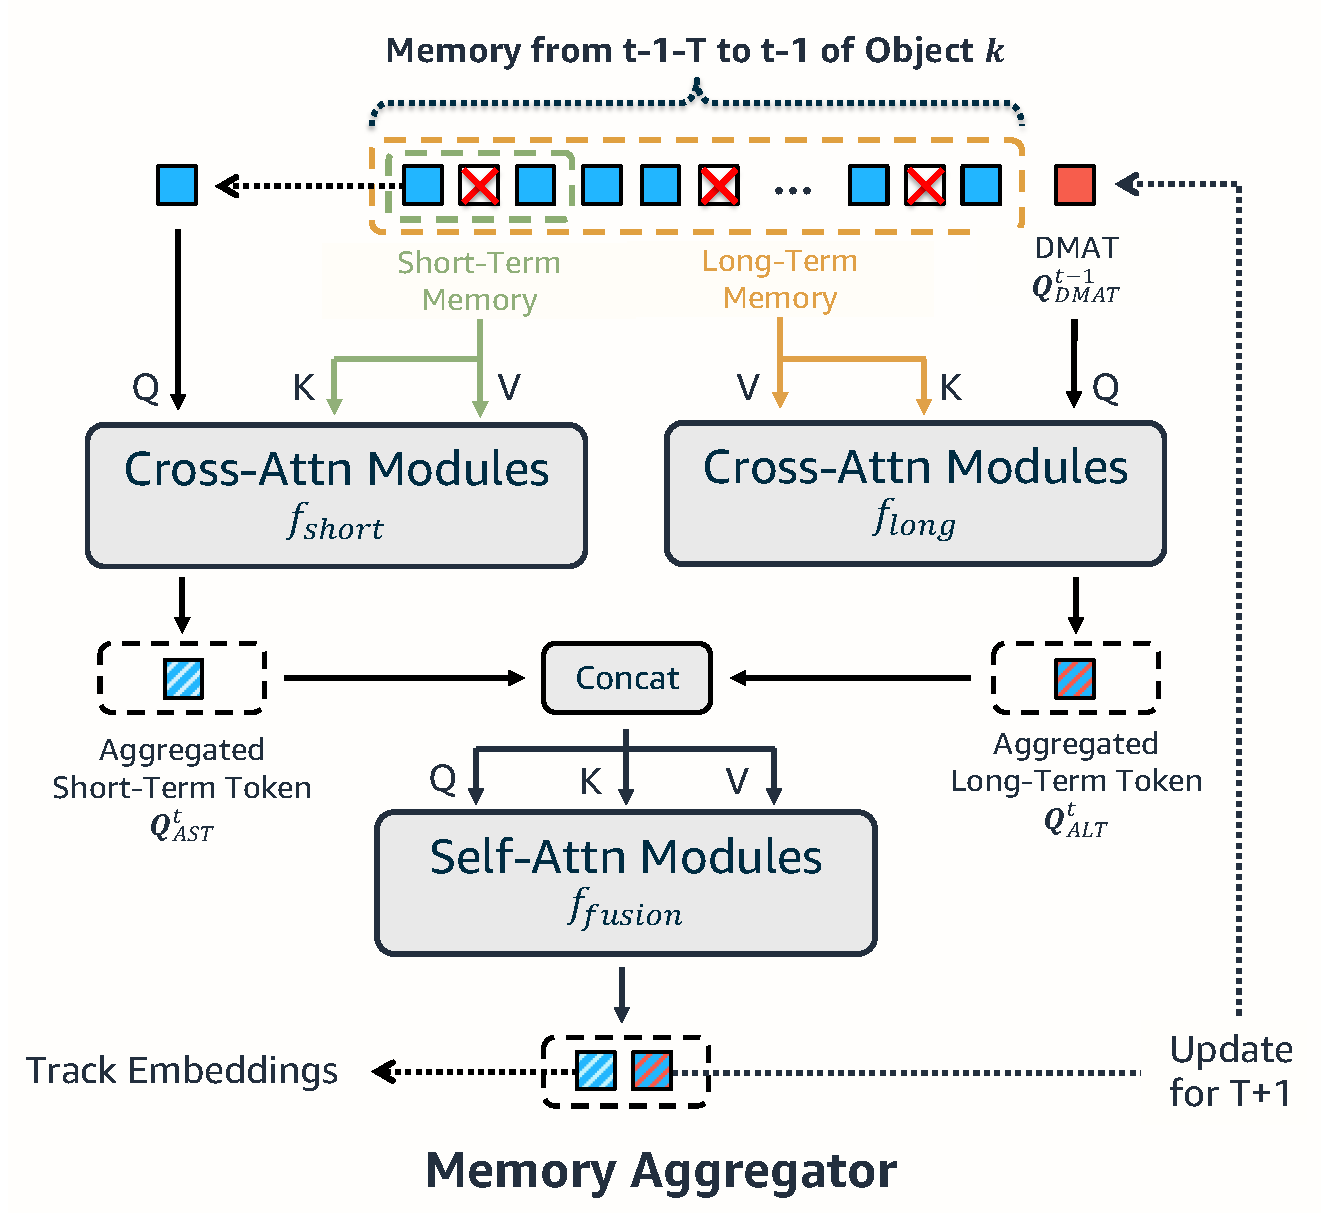
\includegraphics[width=0.5\textwidth]{figures/memory_module.pdf}
    \vspace{-7.5mm}
    \caption{
        \textbf{Illustration of Memory Aggregator}, which consists three attention modules: 1) short-term $f_{short}$ that smoothes out noises in recent frames, 2) long-term $f_{long}$ that extracts supportive features from long-range context, and 3) fusion blocks that aggregate short- and long-term branches. The aggregated embeddings will be used as the track embeddings (blue-white query) and update DMAT (blue-red query) for the next time step.
        % \textbf{Illustration of Memory Aggregator}, which consists three attention modules: 1) a short-term $f_{short}$, 2) a long-term $f_{long}$, and 3) a fusion block. The aggregated embeddings will be used as the track embeddings (blue-white query) and update DMAT (blue-red query) for the next time step.
    }
    \label{fig:ta}
    \vspace{-4.5mm}
\end{figure}

\subsection{Spatio-Temporal Memory}
\label{sec:method:memory}

We store the history states of all $N$ tracked objects in a spatio-temporal memory buffer $\mathbi{X} \in \mathbb{R}^{N \times T \times d}$.
It reserves at most $N_{max}$ objects and a maximum of $T_{max}$ time steps for each object.
The memory is implemented with a first-in-first-out (FIFO) data structure. 
At time step $t$, the memory is represented as the states of $N_{tck}^{t-1}$ active objects in the past $T$ frames, $\mathbi{X}^{t-1-T:t-1}=\{x_k^{t-1-T:t-1}\}_{k=1:N_{tck}^{t-1}}$, where $x_k^{t-1-T:t-1}$ is the states of the $k$-th object and is padded with $\mathbi{0}$ if this object does not appear in the frame $I^t$.
When $T$ is larger than $T_{max}$, the ``oldest'' state $x_k^{t-1-T}$ of each tracklet graduates from the memory.
$N_{max}$ is set to be significantly large (\eg, 300 or 600) to cover the typical number of objects in a video, and a choice of $T_{max}$ is 24.

\subsection{Memory Encoding}
\label{sec:method:theta_E}

As shown in Fig.~\ref{fig:ta}, we encode the memory and extract the track embedding with three attention modules:
1) a short-term block $f_{short}$ for assembling embeddings of neighboring frames to smooth out the noises,
2) a long-term block $f_{long}$ for extracting relevant features in the temporal window covered by the memory,
and 3) a fusion block $f_{fusion}$ for aggregating embeddings from short- and long-term branches.

For each tracklet, the short-term module $f_{short}$ takes as inputs its previous $T_s$ states while the long-term memory module $f_{long}$ utilizes longer history with length of $T_l$ ($T_s \ll T_l$).
$f_{short}$ and $f_{long}$ are implemented with multi-head cross-attention modules, where the history states are key and value inputs.
% We assume that the observations in the current frame are closer to those in the nearby frames and the long-term memory contains more redundant but supportive information.
The input query for $f_{short}$ is the most recent state $\mathbi{X}^{t-1}$, while an dynamically updated embedding, called \textit{Dynamic Memory Aggregation Tokens (DMAT)}, $\mathbi{Q}^{t-1}_{dmat} = \{{q_{dmat}}_k^{t-1}\}_{k=1:N_{tck}}$ is used for $f_{long}$.
When every tracklet is initiated, it is associated with the same DMAT as others; after that, at time step $t > 0$, DMAT is iteratively updated from the previous step. This design will be further validated in Sec.~\ref{sec:exp:ablation}.
The outputs of the short- and long-term branches, denoted as \textit{Aggregated Short-term Token (AST)} $\mathbi{Q}^t_{AST}$ and \textit{Aggregated Long-term Token (ALT)} $\mathbi{Q}^t_{ALT}$, are then fused by $f_{fusion}$.
It outputs the track embedding $\mathbi{Q}_{tck}^t$ and an updated $\mathbi{Q}^{t}_{dmat}$ where the latter is retained for the next timestep. 

\subsection{Memory Decoding}
\label{sec:method:theta_D}

The memory decoder $\Theta_D$ takes the proposal embedding, track embedding, and the image feature as inputs to produce the final tracking results. 
It is realized by using stacked Transformer decoder units, where the concatenated proposal and track embeddings $[\mathbi{Q}^t_{pro}, \mathbi{Q}^t_{tck}]$ are used as queries.
$\Theta_D$ takes the encoded image feature $z_1^t$ from $\Theta_H$ as key and value.

For each entry $q_i^t$ in $\Theta_D$'s outputs $[\widehat{\mathbi{Q}}^t_{pro}, \widehat{\mathbi{Q}}^t_{tck}]$, the decoding process generates three predictions: the bounding box (in the format of offsets \wrt the learned reference points), the \emph{objectness score}, and the \emph{uniqueness score}.
The objectness score $o_{i}^t$ for a query $q_i^t$ ranges from $0$ to $1$, where $o_{i}^t=1$ means the model determines the entry is depicting a visible object.
The uniqueness score $u_i^t$ also ranges from $0$ to $1$. When $u_i^t=1$ the model predicts that the object depicted by $q_i^t$ is unique and should be included in the tracking outputs. Otherwise it needs to be suppressed. We define that $u_i^t=1$ if $q_i^t\in \widehat{\mathbi{Q}}^t_{tck} $. When the model learns to predict $u_i^t$ for each proposal entry, we enforce that a proposal is only considered novel ($u_i^t=1$) when it is not related to any object being tracked. 
We can then define a unified \textbf{confidence score} for both proposal and track entries as the multiplication of objectiveness and uniqueness scores:
% as $s_k^t = o_k^t \cdot u_k^t$:
%
\vspace{-1.0mm}
\begin{equation}
s_k^t = 
    o_k^t \cdot u_k^t.
\label{eq:score}
\end{equation}
\vspace{-1.0mm}
%
The predicted confidence scores of the proposal and track queries are referred to as $\mathbi{S}^t_{tck}$ and $\mathbi{S}^t_{pro}$, respectively. 
For each entry $q_i^t$, the model predicts its bounding box $\mathbf{b}_i^t$, where $\mathbf{b}_i^t \in \mathbb{R}^{4 \times 1}$ includes the object's center coordinates, width, and height. 

The above formulation allows us to solve the object detection and data association problem simultaneously.
In inference, we threshold each entry of $[\widehat{\mathbi{Q}}^t_{pro}, \widehat{\mathbi{Q}}^t_{tck}]$ with the threshold $\epsilon$ and only retain entries with $s_i^t \ge \epsilon$. The resulted entries will automatically bear an track identity or initialize a new track according to whether they come from  $\widehat{\mathbi{Q}}^t_{pro}$ or $\widehat{\mathbi{Q}}^t_{tck}$.
We can then obtain the final tracking results by combining the inherited or newly formed track identities with the corresponding bounding box prediction. There is \emph{no} need for further post processing~\cite{wojke2017simple,bergmann2019tracking,zhang2020fair}. 

To generate the supervision signals for $o_i^t$, $u_i^t$, and $\mathbf{b}_i^t$ on each frame, we first assign the objectiveness score and bounding box to entries in $\widehat{\mathbi{Q}}^t_{tck}$ based on whether the tracked object is present in this frame. 
Then for each entry in $\widehat{\mathbi{Q}}^t_{pro}$, we assign the groundtruth bounding boxes, regardless of new or already tracked, to each entry through bipartite matching~\cite{erhan2014scalable,carion2020end}.
Then we assign the groundtruth uniqueness score to each proposal entry, as shown in Fig.~\ref{fig:asso_solver}, based on whether its matched object has been seen before. 

\begin{figure}
    \centering
    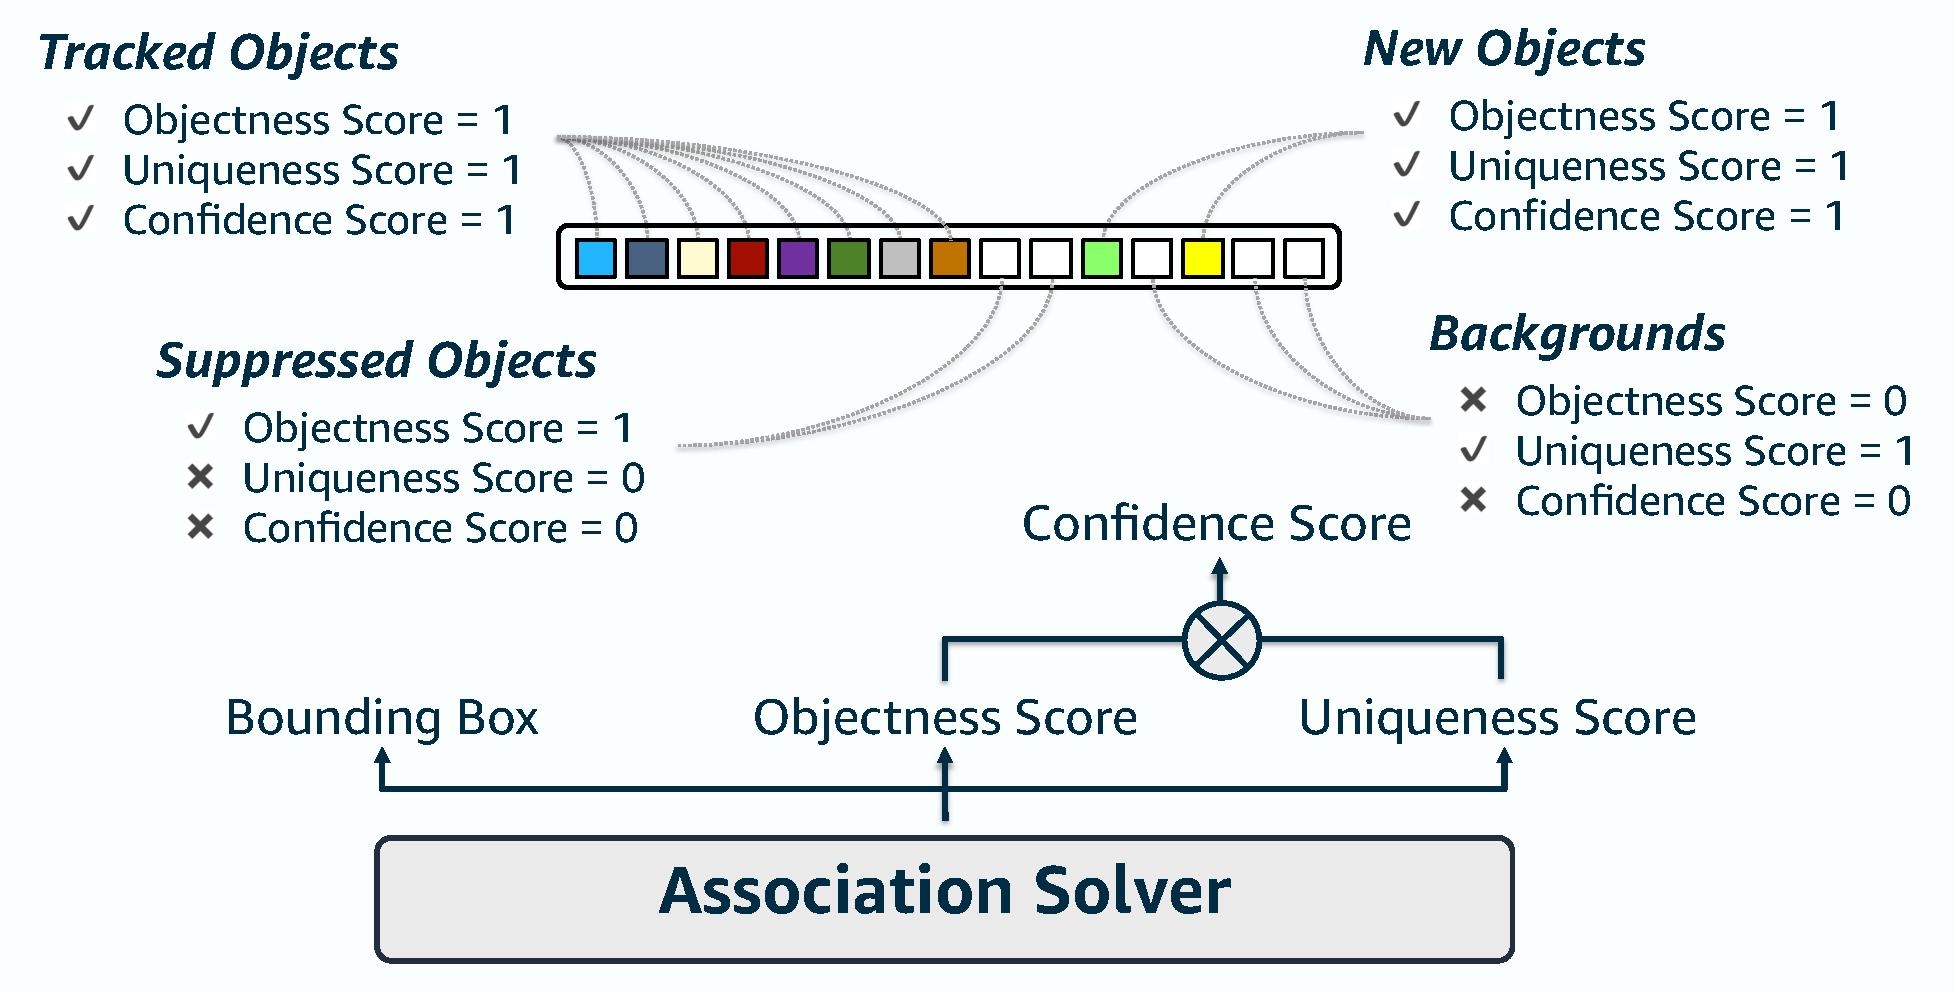
\includegraphics[width=0.5\textwidth]{figures/asso_module.pdf}
    \vspace{-6.0mm}
    \caption{\textbf{Illustration of ground truth assignment} to tracked objects, new objects, suppressed objects, and backgrounds. We show the assigned groundtruth scores for each type of entry.}
    \label{fig:asso_solver}
    \vspace{-4.0mm}
\end{figure}

\subsection{Training MeMOT}
\label{sec:method:training}

We supervise MeMOT with the \textit{tracking loss} computed on the $o_i^t$, $u_i^t$, $\mathbf{b}_i^t$ following the assignment process above as
%
\begin{equation}
%\small
    L_{tck} = \lambda_{cls}(L'_{obj}+L'_{uni})+\lambda_{L_1}L'_{bbox}+\lambda_{iou}L'_{iou},
\end{equation}
%
where $\lambda$s are hyper-parameters for weight scaling, $L_{obj}$ and $L_{uni}$ are focal loss on objectness scores and uniqueness scores, $L_{bbox}$ is L1 loss for bounding box regression, $L_{iou}$ is the generalized IoU loss~\cite{rezatofighi2019generalized}.

Additionally, we apply a detection loss to the proposal embedding similar to Deformable DETR's~\cite{zhu2020deformable} to enhance MeMOT's localization capability.
Specifically, we attach an auxiliary linear decoder to the proposal embedding to output bounding boxes and object classification scores. We then assign the object instances to them as in normal object detection tasks~\cite{zhu2020deformable} and similarly compute the loss as
%
\begin{equation}
%\small
   L_{det} = \lambda_{cls}L_{obj}+\lambda_{L_1}L_{bbox}+\lambda_{iou}L_{iou}.
\end{equation}
%
Note the auxiliary decoder is discarded after training. 

% , which is matched by the Hungarian algorithm, while those for the $\Theta_D$'s are determined by object identities (\ie, each query is responsible for a track).
% Formally, given the prediction results from the $\Theta_H$ decoder and $\Theta_D$ as $\hat{Y}_\tau$ and $\hat{Y'}_\tau$, respectively, their \textit{matched} ground truths are $Y_\tau$ and $Y'_\tau$ (depending on whether the object identity is considered), the losses are formulated as:
% %
% \begin{equation}
% \footnotesize
%     \begin{split}
%     L_{det}(Y_i,\hat{Y}_i) = &\lambda_{cls}L_{obj}+\lambda_{L_1}L_{bbox}+\lambda_{iou}L_{iou}, \\ 
%      L_{tck}(Y'_i,\hat{Y'}_i) = & \lambda_{cls}(L'_{obj}+L'_{uni})+\lambda_{L_1}L'_{bbox}+\lambda_{iou}L'_{iou},
%     \end{split}
% \end{equation}
% %
% where $\lambda$s are hyper-parameters for weight scaling, $L_{obj}$ and $L_{uni}$ are focal loss on objectness scores and uniqueness scores, $L_{bbox}$ is L1 loss for bounding box regression, $L_{iou}$ is the generalized IoU loss~\cite{rezatofighi2019generalized}.

%$L_{cls}$ is the objectness score $\hat{Y}_i$ and confidence score for $\hat{Y'}_i$ (defined in Eq.~\ref{eq:score}).

Following MOTR~\cite{zeng2021motr}, we compute the tracking loss in a clip by the sum of all individual track queries' losses normalized by the total number of object instances.
For a clip with $T$ frames, the overall loss $L_{clip}$ is a combination of the tracking loss and auxiliary detection loss as:
%
\begin{equation}
    \footnotesize
    \begin{split}
    L_{clip} &= \lambda_{tck}L_{clip-tck}+\lambda_{det}L_{clip-det} \\
    &=\frac{\lambda_{tck}}{\sum_{t=0}^{T} N_t}\sum_{t=0}^T\sum_{i=0}^{|\mathbi{Q}^t_{tc}, \mathbi{Q}^t_{pro}|}{L_{tck}^{(i, t)}}+\frac{\lambda_{det}}{T}\sum^T_{t=0}\frac{1}{N_t}\sum_{j=0}^{|\mathbi{Q}^t_{pro}|}L_{det}^{(j, t)},
    \end{split}
    \label{eq:cliploss}
\end{equation}
%
where $\lambda_{tck} \in \mathbb{R}$ and $\lambda_{det} \in \mathbb{R}$ are the loss weights for balancing the tracking loss and the auxiliary detection loss, respectively. 
Here $N_t$ denotes the total number of visible objects in the frame at time $t$.

%(\ie, new objects plus tracked objects) of bounding boxes in frame $t$.